\documentclass[8pt]{article}

\usepackage[a4paper,landscape,margin=0.7cm]{geometry}
\usepackage{multicol}
\usepackage{listings}
\usepackage{titlesec}
\usepackage{xcolor}
\usepackage{graphicx}

\lstdefinestyle{Cstyle}{
language=C,
basicstyle=\ttfamily\scriptsize,
keywordstyle=\color{blue}\bfseries,
stringstyle=\color{red},
commentstyle=\color{green!50!black},
numbers=none,
breaklines=true,
columns=fullflexible,
showstringspaces=false
}

\lstset{style=Cstyle}
\setlength{\parindent}{0pt}
\setlength{\parskip}{2pt}

\titleformat{\section}{\small\bfseries}{}{0em}{}

\lstset{
language=C,
basicstyle=\ttfamily\scriptsize,
breaklines=true,
columns=fullflexible
}

\begin{document}


\begin{multicols*}{3}
\raggedcolumns

%%%%%%%%%%%%%%%%%%%%%%%%%%%%%%%%%%%%%%%%
Stats on a FILE with Read

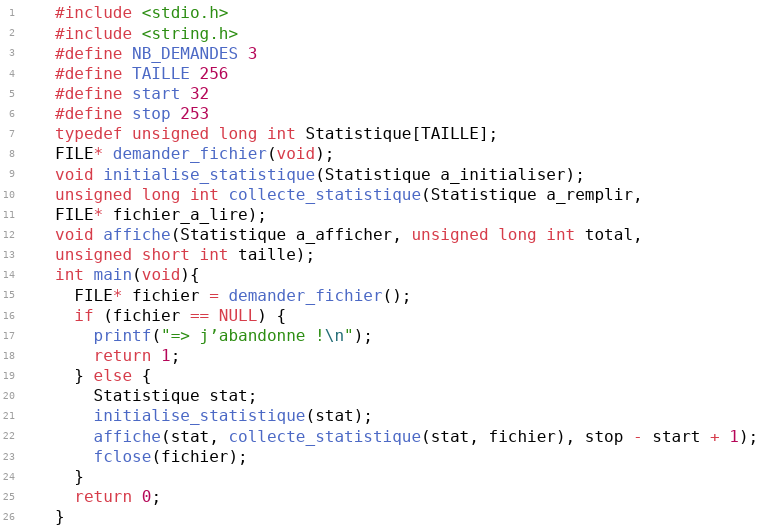
\includegraphics[width=\linewidth]{images/img_20260316_170631.png}

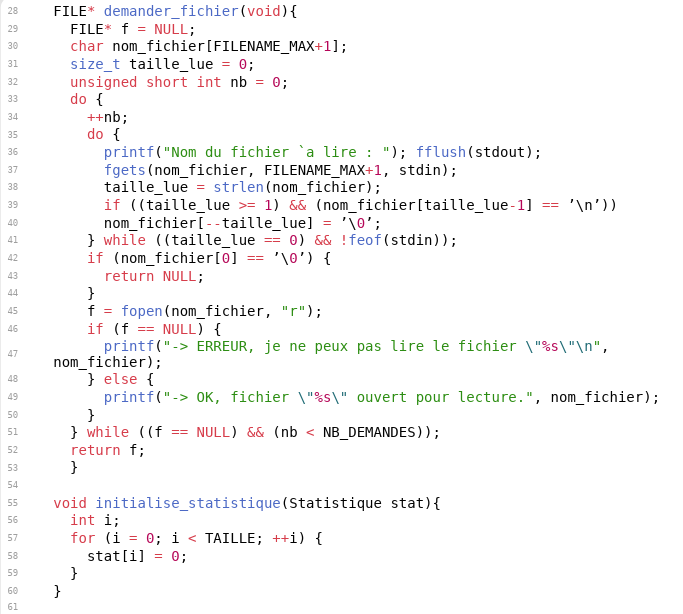
\includegraphics[width=\linewidth]{images/img_20260316_171233.png}

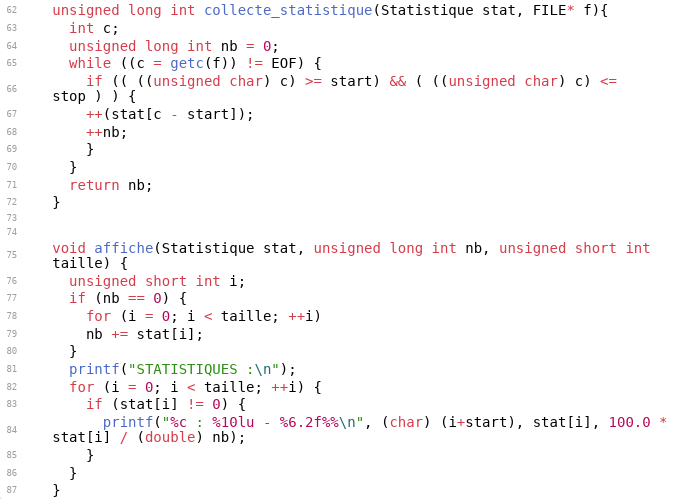
\includegraphics[width=\linewidth]{images/img_20260316_171301.png}

Vector
\begin{lstlisting}[language=C]
#include <stdlib.h>
#include <stdint.h>

typedef int type_el;

typedef struct {
  size_t size;      // nb d'elem utilisees
  size_t allocated; // capacitee allouee
  type_el* content; // zone allouee dynamiquement
} vector;

#define VECTOR_PADDING 128

#ifndef SIZE_MAX
#define SIZE_MAX (~(size_t)0)
#endif

vector* vector_construct(vector* v) {
  if (v != NULL) {
    vector result = (vector){0,0,NULL};
    result.content = calloc(VECTOR_PADDING,sizeof(type_el));
    if (result.content == NULL) return NULL;
    result.allocated = VECTOR_PADDING;
    *v = result;
  }
  return v;
}

void vector_delete(vector* v) {
  if (v != NULL && v->content != NULL) {
    free(v->content);
    v->content = NULL;
    v->size = 0;
    v->allocated = 0;
  }
}

vector* vector_enlarge(vector* v) {
  if (v != NULL) {
    vector result = *v;
    result.allocated += VECTOR_PADDING;

    if (result.allocated > SIZE_MAX/sizeof(type_el)) return NULL;

    type_el* temp =
      realloc(result.content,result.allocated*sizeof(type_el));
    if (temp == NULL) return NULL; // v inchangé

  result.content = temp; // si succes de reall. on maj le pointeur
  *v = result;
  }
  return v;
}

size_t vector_push(vector* v,type_el val) {
  if (v != NULL) {
    while (v->size >= v->allocated) {
      if (vector_enlarge(v) == NULL) return 0;
    }
    v->content[v->size] = val;
    ++(v->size);
    return v->size;
  }
  return 0;
}
\end{lstlisting}

Allocation tableau dynamique
\begin{lstlisting}
1D
t_type* arr = calloc(n, sizeof(t_type));
if(arr == NULL)return NULL;
free(arr);

2D
double** m = calloc(rows, sizeof(double*));
if(m==NULL)return NULL;
for(size_t l = 0; l < rows; l++)){
  m[l] = calloc(cols, sizeof(double));
  if(m[l]==NULL){ // on supprime les lignes deja allouees
    for(int t = (int)l; t>=0;--t){
      free(m[t]);
      m[t] = NULL;
    }
    free(m); m = NULL; return NULL
  }
}
//Libération ordre inverse
for(size_t i = 0; i < rows; i++){
  free(m[i]);
  m[i] = NULL;
}
free(m);
m = NULL;

<- Alloc, d'une struct contenant tableau dyn 
\end{lstlisting}
Realloc safe
\begin{lstlisting}
// toujours passer par un temporaire
t_type* temp = realloc(arr- >elements, new_size * sizeof(t_type));
if (temp == NULL) {
  // arr->elements est toujours valide ici ! (abandon)
  free(arr->elements);
  free(arr);
  return -1;
}
arr->elements = temp; // seulement si succès
// ⚠ NE PAS free(temp) après arr->elements = temp :
// les deux pointeurs pointent vers le même bloc !
  
\end{lstlisting}

\section{Write to a file}
\begin{lstlisting}
#include <stdio.h>
#include <string.h>

/* taille maximale pour un nom */
#define TAILLE_NOM 1024

int main(void)
{
    char const nom_fichier[] = "data.dat"; /* le nom du fichier */
    FILE* sortie;
    int taille_lue;

    char nom[TAILLE_NOM+1];   /* pour stocker le "nom" à lire depuis le clavier */
    unsigned int age;         /* pour stocker l'"age" à lire depuis le clavier */

    /* Ouverture de data.dat en écriture (w=write) */
    sortie = fopen(nom_fichier, "w");

    /* on teste si l'ouverture du flot s'est bien réalisée */
    if (sortie == NULL) {
        fprintf(stderr,
                "Erreur: le fichier %s ne peut etre ouvert en écriture !\n",
                nom_fichier);
        return 1; /* retourne un autre chiffre que 0 car il y a eu une erreur */
    }

    /* itération sur les demandes à entrer :
       on continue tant que stdin est lisible */
    while (!feof(stdin)) {

        /* tant qu'un nom vide est entré */
        do {
            printf("Entrez un nom (CTRL+D pour terminer) : ");
            fflush(stdout);

            fgets(nom, TAILLE_NOM+1, stdin);

            taille_lue = strlen(nom) - 1;
            if ((taille_lue >= 0) && (nom[taille_lue] == '\n'))
                nom[taille_lue] = '\0';

        } while (!feof(stdin) && (taille_lue < 1));

        if (!feof(stdin)) {

            /* L'utilisateur a bien saisi un nom,
               on peut donc lui demander de saisir l'age. */
            printf("âge : ");
            fflush(stdout);

            taille_lue = scanf("%u", &age);

            if (taille_lue != 1) {
                printf("Je vous demande un age (nombre entier positif) pas "
                       "n'importe quoi !\nCet enregistrement est annulé.\n");

                while (getc(stdin) != '\n'); /* vide le tampon d'entrée */
            }
            else {
                getc(stdin); /* récupère le \n résiduel */

                /* écriture dans le fichier */
                fprintf(sortie, "%s %d\n", nom, age);
            }
        }
    }

    /* purisme : retour à la ligne pour finir proprement la question */
    putchar('\n');

    fclose(sortie); /* fermeture du fichier */

    return 0;
}
  
\end{lstlisting} 

Linked Lists
\begin{lstlisting}
#include <stdio.h>
#include <stdlib.h>

#define LISTE_VIDE NULL
#define est_vide(L) ((L) == LISTE_VIDE)

#define type_el int
#define affiche_el(T) printf("%d", (T))

typedef struct Element Element;
typedef Element* ListeChainee;

struct Element {
    type_el valeur;
    ListeChainee suite;
};

void insere_entete(ListeChainee* liste, type_el val) {
    ListeChainee tmp = *liste;

    *liste = malloc(sizeof(Element));
    if (*liste != NULL) {
        (*liste)->valeur = val;
        (*liste)->suite = tmp;
    } else {
        *liste = tmp;
    }
}

void insere_apres(Element* e, type_el val) {
    Element* n = malloc(sizeof(Element));
    if (n != NULL) {
        n->valeur = val;
        n->suite = e->suite;
        e->suite = n;
    }
}

void supprime_tete(ListeChainee* liste) {
    if (!est_vide(*liste)) {
        ListeChainee tmp = (*liste)->suite;
        free(*liste);
        *liste = tmp;
    }
}

void supprime_suivant(Element* e) {
    supprime_tete(&(e->suite));
}

size_t taille(ListeChainee liste) {
    size_t t = 0;
    while (!est_vide(liste)) {
        ++t;
        liste = liste->suite;
    }
    return t;
}

void affiche_liste(ListeChainee liste) {
    ListeChainee i;
    putchar('(');
    for (i = liste; !est_vide(i); i = i->suite) {
        affiche_el(i->valeur);
        if (!est_vide(i->suite)) printf(", ");
    }
    putchar(')');
}
\end{lstlisting}

Ecriture dans fichier (scanf)
\begin{lstlisting}
int process(const char* filename) {
  FILE* file = fopen(filename,"w");
  if (file == NULL) {
    fprintf(stderr, "Impossible d'ouvrir %s\n", filename);
    return -1;
  }
  char name[100];
  int age;
  printf("Enter a name (CTRL+D to finish): ");
  while (scanf("%99s", name) != EOF) {
    printf("age: ");
    if (scanf("%d", &age) != 1 || age < 0) {
      printf("(positive integer)!\n");
      printf("canceled.\n");
      int c; // vider la ligne courante du buffer
      while ((c = getchar()) != '\n' && c != EOF);
    } else {
      fprintf(file, "%s %d\n", name, age);
    }
    printf("Entrer a nane (CTRL+D to finish): ");
  }
  fclose(file);
  return 0;
}
  
\end{lstlisting}


\end{multicols}

\end{document}
